Este capítulo aborda los términos y definiciones a tener en cuenta y sirve como introducción a Active Directory. En primer lugar, se define la forma en la que los Sistemas Windows gestioana la autenticación y la auterización. Posteriormente, se definen los protocolos de seguridad para la verificación de la autenticación NT Lan Manager y Kerberos. Finalmente, se presenta Active Directory y la terminología necesaria relativa a este.\\

\section{Autenticación y Autorización}

Uno de los principales requisitos a la hora de entender como funcionan la mayoría de los ataques contra Sistemas Windows pasa por la gstión de la autenticación y autorización de los usuarios que inician sesión en el ordenador ya sea a nivel local o en red.\\

Por un lado, la \textbf{autenticación} consiste en la verificación de la identidad de un usuario, dicho con otras palabras, que el sistema de autenticación se asegure de que un usuario es quién dice ser. Por ejemplo, conociendo la contraseña del usuario que dice ser.\\

Por otro lado, la \textbf{autorización} consiste en establacer y delimitar los recursos a los que puede acceder, o no puede acceder ya que los tiene restringidos un usuario (o grupos de usuarios).\\


\subsection{Interactive Logon}

El proceso de autenticación a través de inicio de sesión interactivo del inglés {\it Interactive Logon}, a diferencia del inicio de sesión en red o {\it Network Logon}, es llevado a cabo por el proceso {\it WinLogon} que se encarga de recoger las credenciales introducidas por el usuario y su posterior validación. Un usuario que inicia sesión en un equipo ya sea localmente o un inicio de sesión en red introduce el usuario y la contraseña (denominado credenciales de usuario) y sirve para verificar la identidad del usuario. Por otro lado, cuando se inicia sesión a través de una Smart Card {\it (Smart Card Logon)} las credenciales están almacenadas en el chip de la tarjeta y estas son leídas por un dispositivo externo y el usuario introduce el {\it Personal Identification Number (PIN)}~\cite{Capitulo2:Logon}~\cite{Capitulo2:Logon2}.\\

\subsubsection{Proceso WinLogon}

WinLogon es el proceso encargado de coordinar el inicio de sesión. Además, este proceso también se encarga de gestionar el {\it logout}, lanzar los procesos necesarios para la autenticación de un usuario, cambiar las contraseñas, bloquear y desbloquear un equipo y proporcionar la seguridad necesaria para que ningún otro proceso pueda acceder a información sensible cuando estos procedimientos se están llevando a cabo. 

Como se puede ver en la Figura \ref{WinLogon} el proceso de inicio iterativo consta de varias fases~\cite{Capitulo2:WinInternals}:

\begin{figure}[t!] %[ht!] para here [b] para bottom [t] para top
\begin{center}
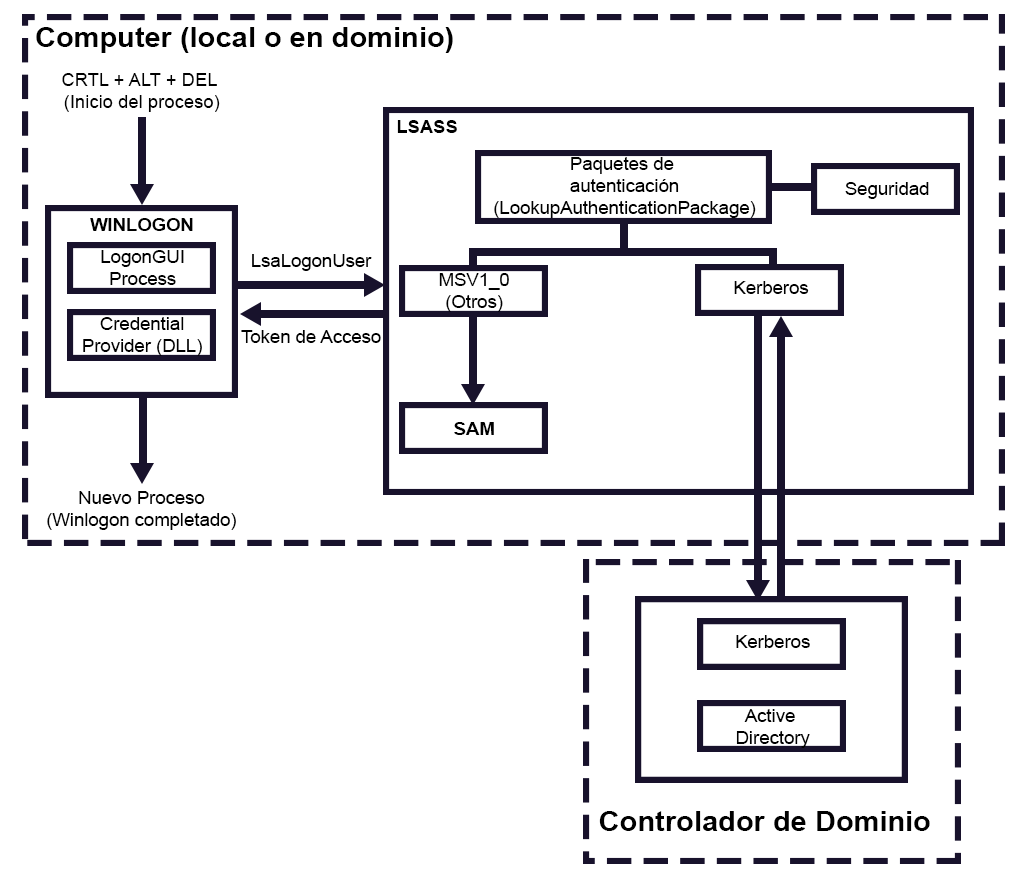
\includegraphics[width=16cm]{WinLogon.png}
\end{center}
\caption{Proceso de inicio de sesión interactivo (WinLogon).}
\label{WinLogon}
\end{figure}

\begin{enumerate}
\item En primer lugar, el proceso de inicio de sesión comienza con una secuencia denominada {\it Secure Attention Sequence (SAS)}, esta secuencia es {\it CTRL + ALT + DEL} por defecto e inicia el proceso WinLogon.

\item Una vez iniciado el proceso WinLogon, este ejecuta el proceso {\it LogonUI} que proporciona la interfaz por defecto para introducir las credenciales y a su vez carga las bibliotecas de enlace dinámico, del inglés {\it Dynamic-Link Library (DLL)} que se encargan de recoger las credenciales y pasarlas al proceso denominado Servicio Subsistema de Autoridad de Seguridad Local del inglés {\it Local Security Authority Subsystem Service} (LSASS). Estas DLLs denominadas {\it Credential Providers} se encuentran en \footnote{\%SystemRoot\%\textbackslash{}System32\textbackslash{}authui.dll} o en \footnote{\%SystemRoot\%\textbackslash{}System32\textbackslash{}SmartcardCredentialProvider.dll} (Si se trata de un inicio de sesión con Smart Cards).

\item Al ejecutarse Winlogon, también se crea un número identificador de seguridad del inglés {\it Security Identifier} (SID),~\cite{Capitulo2:SID} estructura de datos que identifica a un usuario, grupo y cuentas. Cada cuenta en dominio tiene un único SID que le identifica. Los procesos de Windows utilizar el SID asociado en lugar del nombre de usuario o el grupo al que pertenece, este número se pasa como argumento en la llamada {\it LsaLogonUser} y será incluido en el Token de Acceso {\it (Access Token)} si la autenticación se procesa correctamente. 

\item Una vez introducido usuario y contraseña, WinLogon llama al proceso LSASS a través de la función {\it LsaLookupAuthenticationPackage}. Esta función tiene como objetivo obtener los paquetes de autenticación disponibles en el sistema a través de la clave de registro \footnote{HKEY\_LOCAL\_MACHINE\textbackslash{}SYSTEM\textbackslash{}CurrentControlSet\textbackslash{}Control\textbackslash{}Lsa} como se puede observar en la Figura \ref{Registro-Auth}.

\begin{figure}[t!] %[ht!] para here [b] para bottom [t] para top
\begin{center}
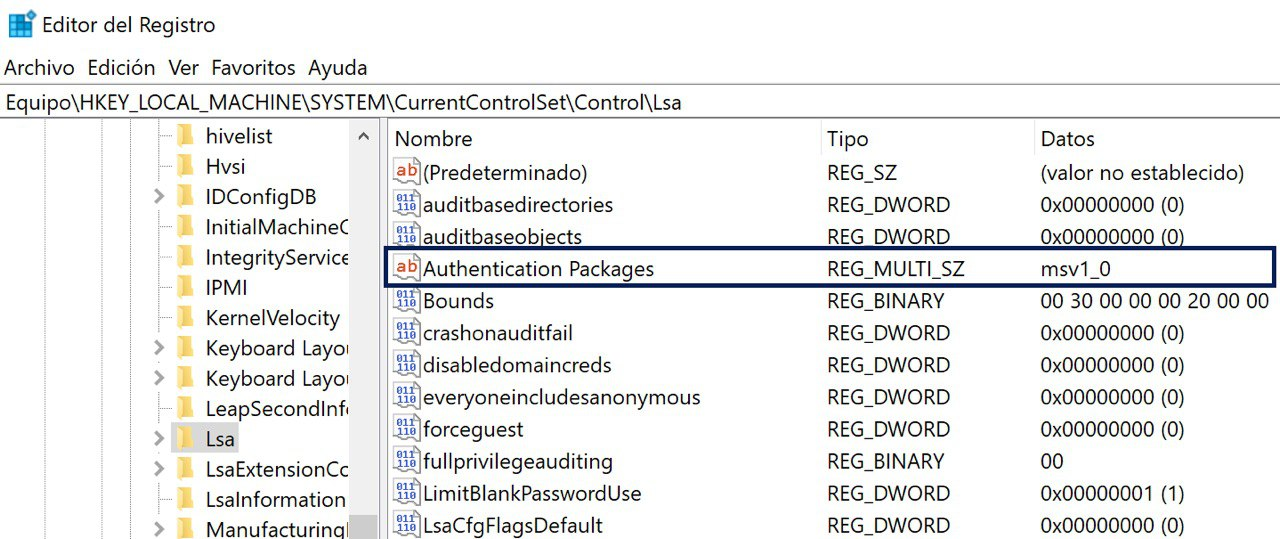
\includegraphics[width=16cm]{Registro-Auth.jpg}
\end{center}
\caption{Clave de registro sobre los paquetes de autenticación.}
\label{Registro-Auth}
\end{figure}

\item Posteriormente, se envían las credendiales a través de la función {\it LsaLogonUser}. Si algún paquete de autenticación autentica el usuario el proceso continua, en cambio, si ningún paquete indica que se ha iniciado sesión correctamente el proceso acaba.

\item Una vez autenticado, el proceso LSASS comprobará en la base de datos de políticas locales si el usaurio autenticado tiene los permisos suficientes para realizar la acción que está solicitando. Si el inicio de sesión no coincide el proceso de autenticación acaba y LSASS elimina cualquier estructura de datos creada y lo notifica a WinLogon. Si el acceso está permitido, LSASS agrega los IDs de seguridad correspondientes, busca en la base de datos los permisos asociados a los usuarios del mismo grupo del SID del usuario y los añade al token de acceso ({\it Access Token}) y crea el Token que será enviado a Winlogon con un mensaje de inicio de sesión correcto. 

\item Por último, Winlogon mira en el registro \footnote{HKLM\textbackslash{}SOFTWARE\textbackslash{}Microsoft\textbackslash{}Windows NT\textbackslash{}Current Version\textbackslash{}Winlogon\textbackslash{}Userinit} y crea un proceso con el valor que haya contenido en el registro. El valor por defecto es {\it Userinit.exe} que carga el perfil del usuario autenticado. 

\end{enumerate}

Una vez definido el proceso de inicio interactivo a grandes rasgos, se va a pasar a detallar los componentes mencionados que forman parte de dicho proceso.

\subsection{Local Security Authority (LSA)}

El subsistema protegido {\it Local Security Authority}~\cite{Capitulo2:LSA} en Sistemas Windows se encarga de validad el acceso a los objetos, comprobar si un usuario tiene permisos suficientes y generar mensajes de auditoría. Es decir, LSA se encarga de las siguientes acciones:

\begin{itemize}
\item Autenticar y registrar los usuarios en un sistema local, es decir, se encarga del proceso visto anteriormente. 
\item Administrar la politica de seguridad local de un sistema, del inglés {\it Local Security Policy}.
\item Proporcionar los servicios necesarios tanto para la autenticación de un usuario, como para la generación de los tokens de acceso correspondientes.
\item Gestionar los servicios necesarios para mantener la relación entre nombres y SIDs.
\end{itemize}

\subsubsection{Local Security Authority Subsystem Service (LSASS)}

El proceso {\it Local Security Authority Subsystem Service (LSASS)} se encarga de instanciar las politicas de seguridad en el sistema, realizar un seguimiento de las políticas de seguridad de las cuentas activas, modificar credenciales y crear tokens de acceso y almacenar las credenciales de los usuarios activos del sitema, esto permite que un usuario no tenga que introducir las credenciales cada vez que accede a un recurso, esto se denomina {\it Single Sign-On}~\cite{Capitulo2:SingleSignOn}.\\

Este proceso es de gran interés para los atacantes ya que LSASS puede almacenar credenciales como Tikets de Kerberos, Hashes NT, Hashes LM o credenciales con algoritmos de cifrado débiles que se puede obtener la contraseña en texto claro.\\

Las contraseñas son almacenadas en LSASS cuando:

\begin{itemize}
\item Se inicia sesión localmente (o remotamente a través de {\it Remote Desktop Protocol (RDP)}). 
\item Se ejecuta un proceso o tarea usando el comando {\it RunAs}.
\item Se ejecuta un servicio de Windows que necesite mayores privilegios de los actuales y se requiere autenticación.
\item Se ejecuta una tarea programada para la que es necesario autenticarse. 
\item Se ejecuta una tarea local usando una herramienta de administración remota. 
\end{itemize}


\subsection{Security Support Provider Interface (SSPI)}

{\it Security Support Provider Interface (SSPI)}~\cite{Capitulo2:SSPI} es una API que permite que una aplicación pueda utilizar varios modelos de seguridad, es decir, abstrae las llamadas necesarias en el proceso de autenticación y permite que una aplicación lleve a cabo un proceso de autenticación sin especificar los protocolos de autenticación, denominados paquetes de autenticación que se verán en detalle en la siguiente sección de este capítulo.\\

En primer lugar, se negocia el protocolo a utilizar, para que el proceso se complete correctamente ambas máquinas deben aceptar mismo {\it Security Support Provider (SSP)}. Un SSP es un DLL que implementa SSPI y permite la ejecució de los paquetes de autenticación. Cada paquete proporciona un "mapeo" entre las llamadas de funciones SSPI de una aplicación y las funciones de un modelo de seguridad.\\

Los principales SPP son: 

\begin{itemize}

\item Kerberos.
\begin{listing}[style=consola, numbers=none]
%SystemRoot\%\Windows\System32\kerberos.dll
\end{listing}

\item NT Lan Manager (NTLM): NTLMv1 y NTLMv2.
\begin{listing}[style=consola, numbers=none]
%SystemRoot%\Windows\System32\msv1_0dll
\end{listing}

\item Digest.
\begin{listing}[style=consola, numbers=none]
%SystemRoot%\Windows\System32\Wdigest.dll
\end{listing}

\item Schanell.
\begin{listing}[style=consola, numbers=none]
%SystemRoot%\Windows\System32\Schannel.dll
\end{listing}

\item Negotiate.
\begin{listing}[style=consola, numbers=none]
%SystemRoot%\Windows\System32\lsasrv.dll
\end{listing}

\end{itemize}

\subsubsection{Negotiate}

Microsoft Negotiate~\cite{Capitulo2:Negotiate} es un SSP que actua como intermediario entre la API SPPI y otro SSP. Cuando una aplicación requiera algún tipo de autenticación, se envía una petición a Negotiate con los armunetos necesarios (parámetros, credenciales, SSPs a utilizar...), este lo examinará y pasará la petición al SSP correspondiente que llevará a cabo la autenticación. \\

Actualmente, Neogtiate elige entre Kerberos y NTLM. Seleccionará el primero simpre y cuando haya conexión entre las dos partes implicadas en el proceso y el usuario haya especificado el Service Principal Name (SPN), un User Principal Name (UPN), o una cuenta de NetBIOS. En cambio, si se trata de una autenticación local utilizará NTLM.

\subsection{Security Account Manager (SAM)}

Uno de los principales elementos que forman parte de la autenticación local es {\it Security Account Manager (SAM)}. La SAM es un archivo que tiene todos los Sistemas Windows y consiste en una base de datos que almacena las credenciales de los usuarios locales. Este fichero almacena el identificador de usuario, nombre de usuario y el hash de la contraseña. Este último puede ser LM o NT. El fichero se encuentra en:

\begin{listing}[style=consola, numbers=none]
%SystemRoot%\Windows\System32\config\SAM
\end{listing}

\subsection{Access Token}

Una vez validada la autenticación, se crea un {\it Access Token}, este objeto describe el contexto de seguridad de un proceso o de un hilo ({\it thread})~\cite{Capitulo2:Access-Token}. Para SSPI se denomina contexto de seguridad a una estructura de datos que contiene datos relevantes de seguridad como puede ser la clave de sesión o la duración de dicha sesión. Cada proceso ejecutado por un usuario dispone de una copia del token de acceso de ese usuario. Windows utiliza estos tokens para identificar a un usuario cuando ejecuta un hilo que necesite privilegios de ese usuario. La información contenida en un {\it Access Token} es:

\begin{itemize}
\item El SID de la cuenta del usuario en cuestión.
\item El SID del grupo de usuarios de los que el usuario es miembro.
\item El SID de la session (logon session).
\item Los privilegios del usuario y del grupo de usuarios al que pertenece.
\item El SID del grupo primario. 
\item El {\it Discretionary Access Control List} (DACL)~\cite{Capitulo2:DACL} por defecto que se utiliza cuando el usuario crea un proceso sin especificar el descriptor de seguridad.
\item La procedencia del token de acceso.
\item Si el token de acceso es primario o es una suplantación. 
\item Una lista de SIDs restrictivos.
\item Niveles de suplatación actuales.
\item Otras estadísticas. 
\end{itemize}

Cuando un administrador local inicia sesión en una máquina, se crean dos tokens diferentes: Un token primario que contendrá el contexto de seguridad del usuario y un token de administrador. Esto es debido a la política de Windows de mínimo privilegio posible, esto significa que el sistema usará por defecto el token primario cuando un proceso o hilo interactue con un {\it Securable Objects}~\cite{Capitulo2:Securable-Objects}. Esto es importante a la hora de entender {\it User Account Control (UAC)}.\\

Para listar las sesiones logon en un sistema se puede utilizar el comando {\it logonsessions} de {\it Windows Sysinternals}~\cite{Capitulo2:Sysinternals} como se puede ver en la Figura \ref{Logonsessions}.

\begin{figure}[t!] %[ht!] para here [b] para bottom [t] para top
\begin{center}
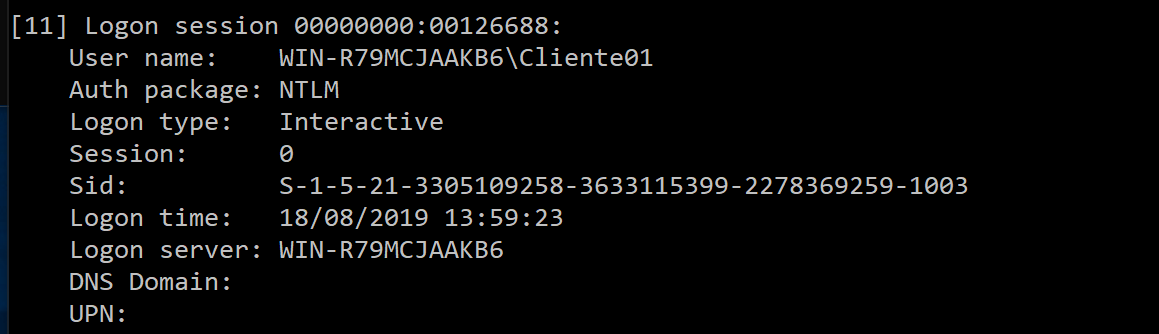
\includegraphics[width=16cm]{Logonsessions.png}
\end{center}
\caption{Salida del comando Logonsessions.}
\label{Logonsessions}
\end{figure}

\subsection{User Account Control (UAC)}

User Account Control (UAC)~\cite{Capitulo2:UAC}~\cite{Capitulo2:UAC2}sirve para controlar cuando se están usando privilegios de adminstración. Como se ha comentado anteriormente al iniciar sesión desde una cuenta administrativa, se crean dos tokens de usuario: uno denominado {\it full access token} y un token secundario denominado {\it filtered access token}. Esto permite que los procesos ejecutados por este usuario se ejecuten con el segundo token siempre y cuando no necesiten privilegios de administración y así cumplir la política de mínimo privilegio posible. Esto lo podemos observar cuando se completa un inicio de sesión válido, el proceso {\it Explorer.exe} se ejecuta con el {\it filtered access token}. Cuando un proceso concreto necesita privilegios de administración, se requerirá una elvación de privilegios realizando una elevación de UAC. Como se puede ver en la Figura \ref{UAC} se ha ejecutado una terminal {\it (cmd.exe)} con privilegios administrativos y aparece el mensaje de Control de Cuentas de Usuario para elevar de privilegios. \\

\begin{figure}[t!] %[ht!] para here [b] para bottom [t] para top
\begin{center}
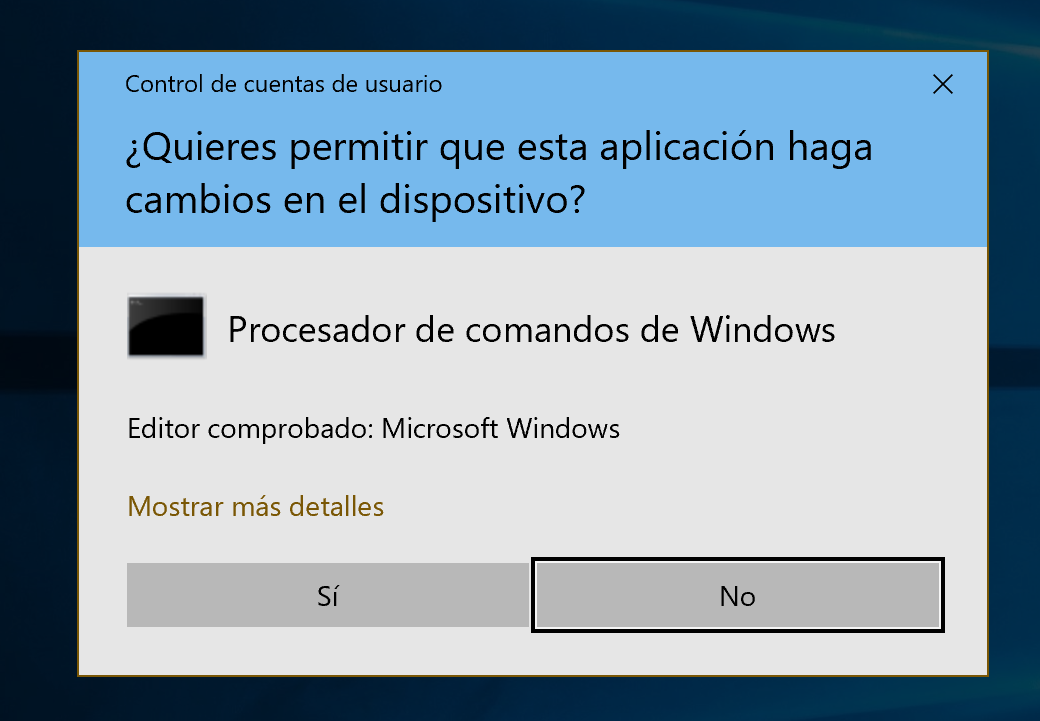
\includegraphics[width=10cm]{UAC.png}
\end{center}
\caption{Control de Cuentas de Usuario al ejecutar cmd.exe}
\label{UAC}
\end{figure}

Para controlar qué procesos necesitan privilegios especiales o cuales no, los Sistemas Windows hacen uso de {\it Mandatory Integrity Control}~\cite{Capitulo2:MIC}, un mecanismo para controlar el acceso a los {\it Securable Objects}~\cite{Capitulo2:Securable-Objects}, para ello, el MIC utiliza niveles de integridad para evaluar el acceso a un proceso. Estos niveles son: {\it untrusted, low, medium, high, system e installer}~\cite{Capitulo2:IntegrityLabels}~\cite{Capitulo2:IntegrityLabels2}. Esto implica que un objeto con integridad baja (low) no puede escribir en un objeto de integridad medio. \\

\begin{itemize}
\item \textbf{Untrusted:} Son aquellos procesos iniciados de forma anónima, como puede ser procesos lanzados desde cuentas de Invitados.  
\item \textbf{Low:} Nivel de integridad usado por defecto para la interacción con internet. Cuando se lanza {\it Internet Explorer} se utiliza este modo, por lo tanto, todos los archivos y procesos asociados a este se le asignan un nivel de integridad bajo.
\item \textbf{Medium:} Nivel de integridad usado por la mayoría de los procesos, es el nivel designado por defecto siempre y cuando no se especifique explícitamente un nivel inferior o superior.
\item \textbf{High:} Nivel de integridad destinado para aquellos procesos que necesitan privilegios de administración. Los objetos con este nivel de integridad solicitarán una elevaciñon de privilegios a través de UAC.
\item \textbf{System:} Nivel de integridad reservado para los objetos del sistema, estos objetos engloban el kernel de Windows y servicios del {\it core}.
\item \textbf{Installer:} Nivel de integridad especial utilizado para la instalación de software. Este nivel es igual o superior a todos los niveles anteiores, lo que permite que este nivel puede desinstalar los demás objetos. 
\end{itemize}

\section{Authentication Packages}

Windows utiliza dos paquetes de autenticación de forma estandar, Kerberos y MSV1\_0. Como se ha comentado anteriormente Microsoft Windows utilizará el paquete MSV1\_0 para sistemas independientes (que no están unidos a un dominio). Este protocolo implementa la versión 2 del protocolo Lan Manager. Además, este paquete se utiliza para sistemas en red unidos a un dominio cuya versión sea anterior a Windows 2000. Por otro lado, el paquete de autenticación Kerberos, se utiliza en sistemas que son parte de un dominio. El paquete de Windows Kerberos se comunicará con un Controlador de Dominio donde se ejecutará y comprobará la validación de las credenciales. Kerberos está desarrolado siguiendo el RFC4120~\cite{Capitulo2:Kerberos}. Los protocolos soportados por ambos paquetes de autenticación serán detallados en los siguientes capítulos.


\subsection{NT Lan Manager (NTLM)}



Como se ha comentado anteriormente, cuando un usuario inicia sesión localmente en Sistemas Windows utiliza el paquete de autenticacióni MSV1\_0~\cite{Capitulo2:MSV10}. LSA llama a este paquete para procesar los datos de inicio de sesión recogidos en el proceso WinLogon para su posterior comprobación con la información contenida en la base de datos SAM. 


En este apartado se va a detallar cómo gestiona Windows el almacenamiento de dichos datos a través de NT Lan Manager (NTLM). \\

\subsection{Windows Hashes}

Para almacenar los contraseñas en la base de datos, los Sistemas Windows utilizan Hashes {\it Lan Manager (LM)} y NT.

\subsubsection{LM}

Los hashes LM son la versión que s


\section{Kerberos}

\section{Active Directory}




